\documentclass{article}

\usepackage[french]{babel} 
\usepackage[T1]{fontenc}
\usepackage{lmodern}
\usepackage[utf8]{inputenc}
\usepackage{array}
\usepackage[bottom]{footmisc}


\usepackage{float}
\usepackage{mathtools}
\DeclarePairedDelimiter{\ceil}{\lceil}{\rceil}
\usepackage{fancyhdr}
\usepackage{extramarks}
\usepackage{amsmath}
\usepackage{amsthm}
\usepackage{amsfonts}
\usepackage{amssymb}
\usepackage{tikz}
\usepackage[plain]{algorithm}
\usepackage{algpseudocode}
\usepackage{algorithmicx}
\usepackage{hyperref}
\usepackage{enumitem}
\graphicspath{ {./figures/} }

%Dessins plz

 \usepackage[usenames,dvipsnames]{pstricks}
 \usepackage{epsfig}
 \usepackage{pst-grad} % For gradients
 \usepackage{pst-plot} % For axes
 \usepackage[space]{grffile} % For spaces in paths
 \usepackage{etoolbox} % For spaces in paths
 \makeatletter % For spaces in paths
 \patchcmd\Gread@eps{\@inputcheck#1 }{\@inputcheck"#1"\relax}{}{}
 \makeatother


\usetikzlibrary{automata,positioning}

%
% Basic Document Settings
%

\topmargin=-0.45in
\evensidemargin=0in
\oddsidemargin=0in
\textwidth=6.5in
\textheight=9.0in
\headsep=0.25in

\linespread{1.1}

\pagestyle{fancy}
\fancyhf{}
%\lhead{\hmwkAuthorName}
\chead{\hmwkClass\ (\hmwkClassInstructor): \hmwkTitle}
\rhead{\firstxmark}
\lfoot{\lastxmark}
\cfoot{\thepage}

\renewcommand\headrulewidth{0.4pt}
\renewcommand\footrulewidth{0.4pt}

%----------------------------------------------------------------------------------------
%   FOOTER FOOTNOTE PATCH
%----------------------------------------------------------------------------------------

\let\origfootrule\footrule
\renewcommand{\footrule}{\iffootnote{}{\origfootrule}}
\renewcommand\footnoterule{\origfootrule}

\setlength\parindent{0pt}


%
% Homework Problem Environment
%
% This environment takes an optional argument. When given, it will adjust the
% problem counter. This is useful for when the problems given for your
% assignment aren't sequential. See the last 3 problems of this template for an
% example.
%
\newenvironment{homeworkProblem}[1][-1]{
    \ifnum#1>0
        \setcounter{homeworkProblemCounter}{#1}
    \fi
    \section{Partie \arabic{homeworkProblemCounter}}
    \setcounter{partCounter}{1}
    \enterProblemHeader{homeworkProblemCounter}
}{
    \exitProblemHeader{homeworkProblemCounter}
}

%
% Homework Details
%   - Title
%   - Due date
%   - Class
%   - Section/Time
%   - Instructor
%   - Author
%

\newcommand{\hmwkTitle}{Rapport TP3}
\newcommand{\hmwkDueDate}{18 novembre 2022}
\newcommand{\hmwkClass}{\ \ IFT 3913}
\newcommand{\hmwkClassTime}{}%Section 
\newcommand{\hmwkClassInstructor}{Professeur: Michalis Famelis}
\newcommand{\hmwkAuthorName}{\textbf{Zi Kai Qin, 20191254\hspace{3cm}Maxime Ton, 20143044}}

%
% Title Page
%

\title{
    \vspace{2in}
    \textmd{\textbf{\hmwkClass:\ \hmwkTitle}}\\
    \normalsize\vspace{0.1in}\small{Pour\ le\ \hmwkDueDate\ à 23:59 }\\
    \vspace{0.1in}\large{\textit{\hmwkClassInstructor\ \hmwkClassTime}}
    \vspace{3in}
}

\author{\hmwkAuthorName}
\date{}

\renewcommand{\part}[1]{\textbf{\large Partie \Alph{partCounter}}\stepcounter{partCounter}\\}

%
% Various Helper Commands
%


%floor and ceiling functions
%\newcommand{\floor}[1]{\left\lfloor #1 \right\rfloor}
%\newcommand{\ceil}[1]{\left\lceil #1 \right\rceil}

% Useful for algorithms
\newcommand{\alg}[1]{\textsc{\bfseries \footnotesize #1}}

% For derivatives
\newcommand{\deriv}[1]{\frac{\mathrm{d}}{\mathrm{d}x} (#1)}

% For partial derivatives
\newcommand{\pderiv}[2]{\frac{\partial}{\partial #1} (#2)}

% Contradiction et limites
\newcommand{\absurde}{\rightarrow \leftarrow}
\newcommand{\tend}{\rightarrow}
\newcommand{\tendUnif}{\xrightarrow{\text{unif}}}
%make this work
%\newcommand{\par}[1]{\xrightarrow{\text{#1}}}



% ensembles
\newcommand{\naturel}{\mathbb{N}}
\newcommand{\entier}{\mathbb{Z}}
\newcommand{\rationnel}{\mathbb{Q}}
\newcommand{\reel}{\mathbb{R}}
\newcommand{\complexe}{\mathbb{C}}
\newcommand{\compl}[1]{\overline{#1}}
\newcommand{\e}{\varepsilon}
\let\emptyset\varnothing


% Integral dx
\newcommand{\dx}{\mathrm{d}x}
\newcommand{\dy}{\mathrm{d}y}
\newcommand{\dt}{\mathrm{d}t}


% Alias for the Solution section header
\newcommand{\solution}{\textbf{\large Solution}}

% Probability commands: Expectation, Variance, Covariance, Bias
\newcommand{\E}{\mathrm{E}}
\newcommand{\Var}{\mathrm{Var}}
\newcommand{\Cov}{\mathrm{Cov}}
\newcommand{\Bias}{\mathrm{Bias}}


%lul
\newcommand{\shrug}[1][]{%
\begin{tikzpicture}[baseline,x=0.8\ht\strutbox,y=0.8\ht\strutbox,line width=0.125ex,#1]
\def\arm{(-2.5,0.95) to (-2,0.95) (-1.9,1) to (-1.5,0) (-1.35,0) to (-0.8,0)};
\draw \arm;
\draw[xscale=-1] \arm;
\def\headpart{(0.6,0) arc[start angle=-40, end angle=40,x radius=0.6,y radius=0.8]};
\draw \headpart;
\draw[xscale=-1] \headpart;
\def\eye{(-0.075,0.15) .. controls (0.02,0) .. (0.075,-0.15)};
\draw[shift={(-0.3,0.8)}] \eye;
\draw[shift={(0,0.85)}] \eye;
% draw mouth
\draw (-0.1,0.2) to [out=15,in=-100] (0.4,0.95); 
\end{tikzpicture}}


%shortcut
\renewcommand{\theenumii}{\arabic{enumii}}
\newcommand{\lra}{\longrightarrow}
\newcommand{\ra}{\rightarrow}
\newcommand{\ifff}{\leftrightarrow}
\newcommand{\Poly}{\mbox{\bf P}}
\newcommand{\NP}{\mbox{\bf NP}}
\newcommand{\NPC}{\mbox{\bf NPC}}
\newcommand{\CNP}{\mbox{\bf Co-NP}}
\newcommand{\R}{\mbox{\bf R}}
\newcommand{\RE}{\mbox{\bf RE}}
\newcommand{\donne}{\stackrel{\hspace{-3pt}*}{|\hspace{-5pt}-\hspace{-5pt}-\
}}

\newtheorem{cor}{Corollaire}
\newtheorem{obs}{Observation}
\newtheorem{con}{Convention}
\newtheorem{dfn}{D\'efinition}
\newtheorem{thm}{Th\'eor\`eme}
\newtheorem{lem}{Lemme}
\newtheorem{prop}{Proposition}
\newtheorem{prob}{Probl\`eme}
\newtheorem{ex}{Exercise}
\newtheorem{rem}{Remarque}
\newtheorem{algo}{Algorithme}


\newcommand{\re}{{\mathbb R}}
\newcommand{\rep}{{\mathbb R}^{> 0}}
\newcommand{\renn}{{\mathbb R}^{\geq 0}}
\newcommand{\nat}{{\mathbb N}}
\newcommand{\intg}{{\mathbb Z}}
\newcommand{\intgp}{\intg^{>0)}}
\newcommand{\intgn}{\intg^{<0)}}
\newcommand{\intgnp}{\intg^{\geq 0}}
\newcommand{\intgnn}{\intg^{\leq 0}}
\newcommand{\barr}{\overline}
\newcommand{\np}{\mbox{{\it NP}}}
\newcommand{\npc}{\mbox{{\it NPC}}}
\newcommand{\cnp}{\mbox{{\it co-NP}}}
\newcommand{\p}{\mbox{{\it P}}}
\newcommand{\cp}{\mbox{{\it co-P}}}
\newcommand{\twobox}{\marginpar{\huge {$\Box$ \hspace{0.5cm}$\Box$} }} 
\newcommand{\repbox}{\marginpar{{\Large \begin{tabular}{|c|}\hline \ \ \
\\ \hline \end{tabular}}} } 
\newcommand{\ssi}{si et seulement si }
\renewcommand{\theprob}{\thesection.\arabic{prob}}
\newcommand{\diam}{{\rm diam}}
\newcommand{\inv}{^{-1}}
\newcommand{\cha}{cha\^\i ne}
\newcommand{\ecc}{{\rm ec}}
\newcommand{\vcc}{{\rm vc}}






\begin{document}
\maketitle
\pagebreak

\section{Introduction:}
Dans le cadre de ce travail pratique, nous allons étudier un échantillon de données portant sur la librarie JFreeChart composée des trois métriques suivantes:
\begin{itemize}
    \item NoCom: nombre de commits
    \item NCLOC: nombre de lignes de code qui ne sont pas ni vides ni commentaires
    \item DCP: densité de commentaires (CLOC/LOC) donnée en pourcentage
\end{itemize}
Nous nous servirons des résultats de cette analyse afin d'évaluer la validité d'une certaine hypothèse donnée.

\section{Partie 1 -- Boîtes à moustache:}

Nous commençons par visualiser notre échantillon à l'aide de boîtes à moustaches.
Ceci requiert quelques calculs, que nous effectuons à l'aide d'Excel\footnote{Voir jfreechart-stats.xlsx}, selon la technique d'analyse vue aux diapositives 7.
Ces calculs nous donnent les valeurs suivantes:
\begin{center}
\begin{tabular}{ c c c c }
 & NoCom & NCLOC & DCP \\
m & 5 & 71.5 & 59.21\\
u & 9 & 180 & 82.31\\
l & 3 & 12 & 49.27\\
d & 6 & 168 & 33.04\\
s & 18 & 432 & 131.87\\
Min & 2 & 4 & 25.24\\
i & 2(-6) & 4(-240) & 25.24(-0.29)\\
Max & 32 & 2732 & 93.44
\end{tabular}
\\
\end{center}
Ces données, nous permettent de construire les boîtes à moustaches suivantes\footnotemark{}:\newline
\footnotetext{Boîtes à moustaches créées sur le site https://www.imathas.com/stattools/boxplot.html}
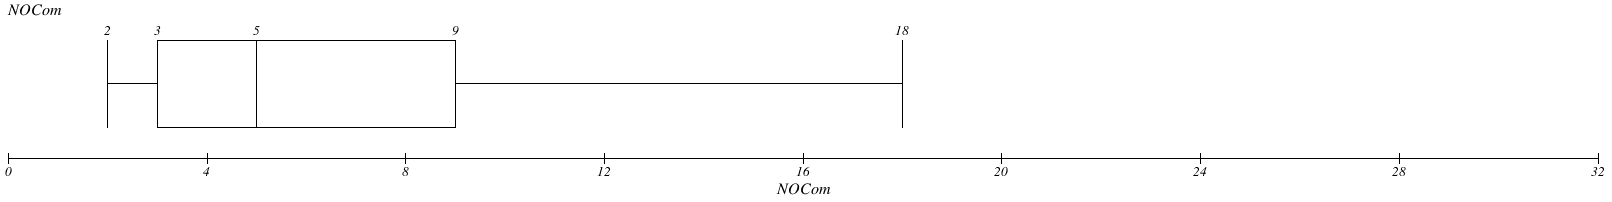
\includegraphics[width=\textwidth]{t1nocom.PNG}
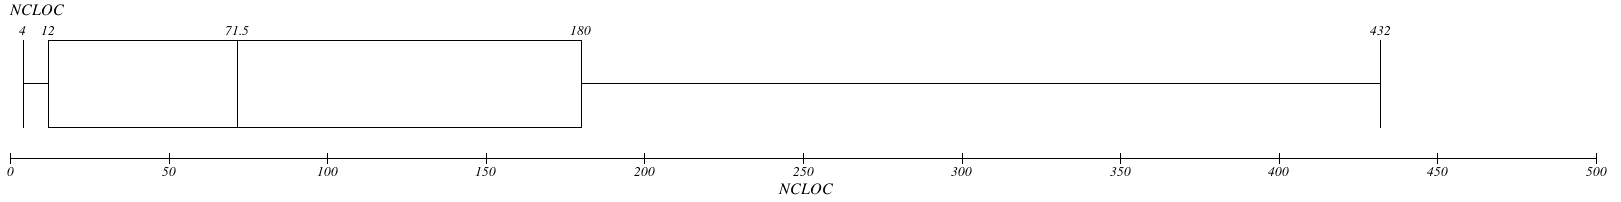
\includegraphics[width=\textwidth]{t1ncloc.PNG}
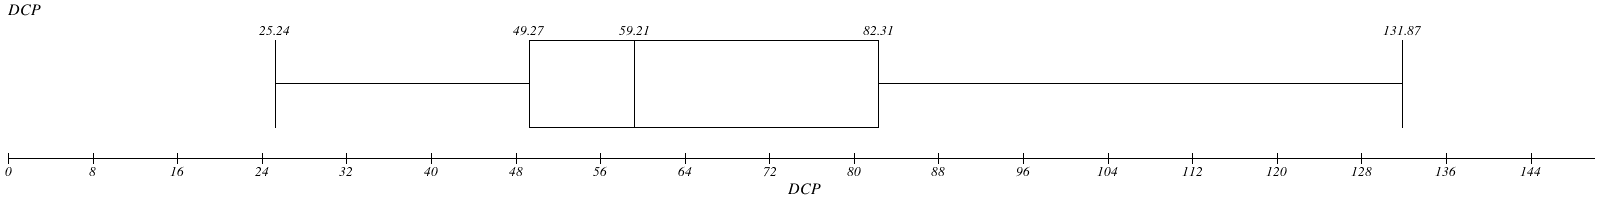
\includegraphics[width=\textwidth]{t1dcp.PNG}
\textbf{NoCom:}
La distribution est biaisée vers le bas avec un quartile supérieur deux fois plus long que le quartile inférieur.
Plusieurs points extrêmes existent au-delà de l'intervalle théorique, particulièrement un point extrème maximum de 32.\newline
\textbf{NCLOC:}
Tout comme NoCom, la distribution est biaisée vers le bas avec un quartile supérieur plus long que le quartile inférieur.
La dispersion est cependant beaucoup plus élevée.
Il y a plusieurs points extrèmes au-delà de la limite supérieure de 432, notamment un maximum de 2732.\newline
\textbf{DCP:}
Encore une fois, le quartile supérieur est beaucoup plus long que le quartile inférieur.
Cependant, l'intervalle théorique est plus centré et les valeurs sont moins dispersées.
Il n'y a pas points extrèmes.

\vspace*{\fill}
\section{Partie 2 -- Études de corrélations:}

Nous cherchons maintenant à étudier la corrélation entre les différentes métriques.
L'outil \emph{Trendline} de Google Sheets nous permet de générer les droites de régression:\newline
\begin{center}
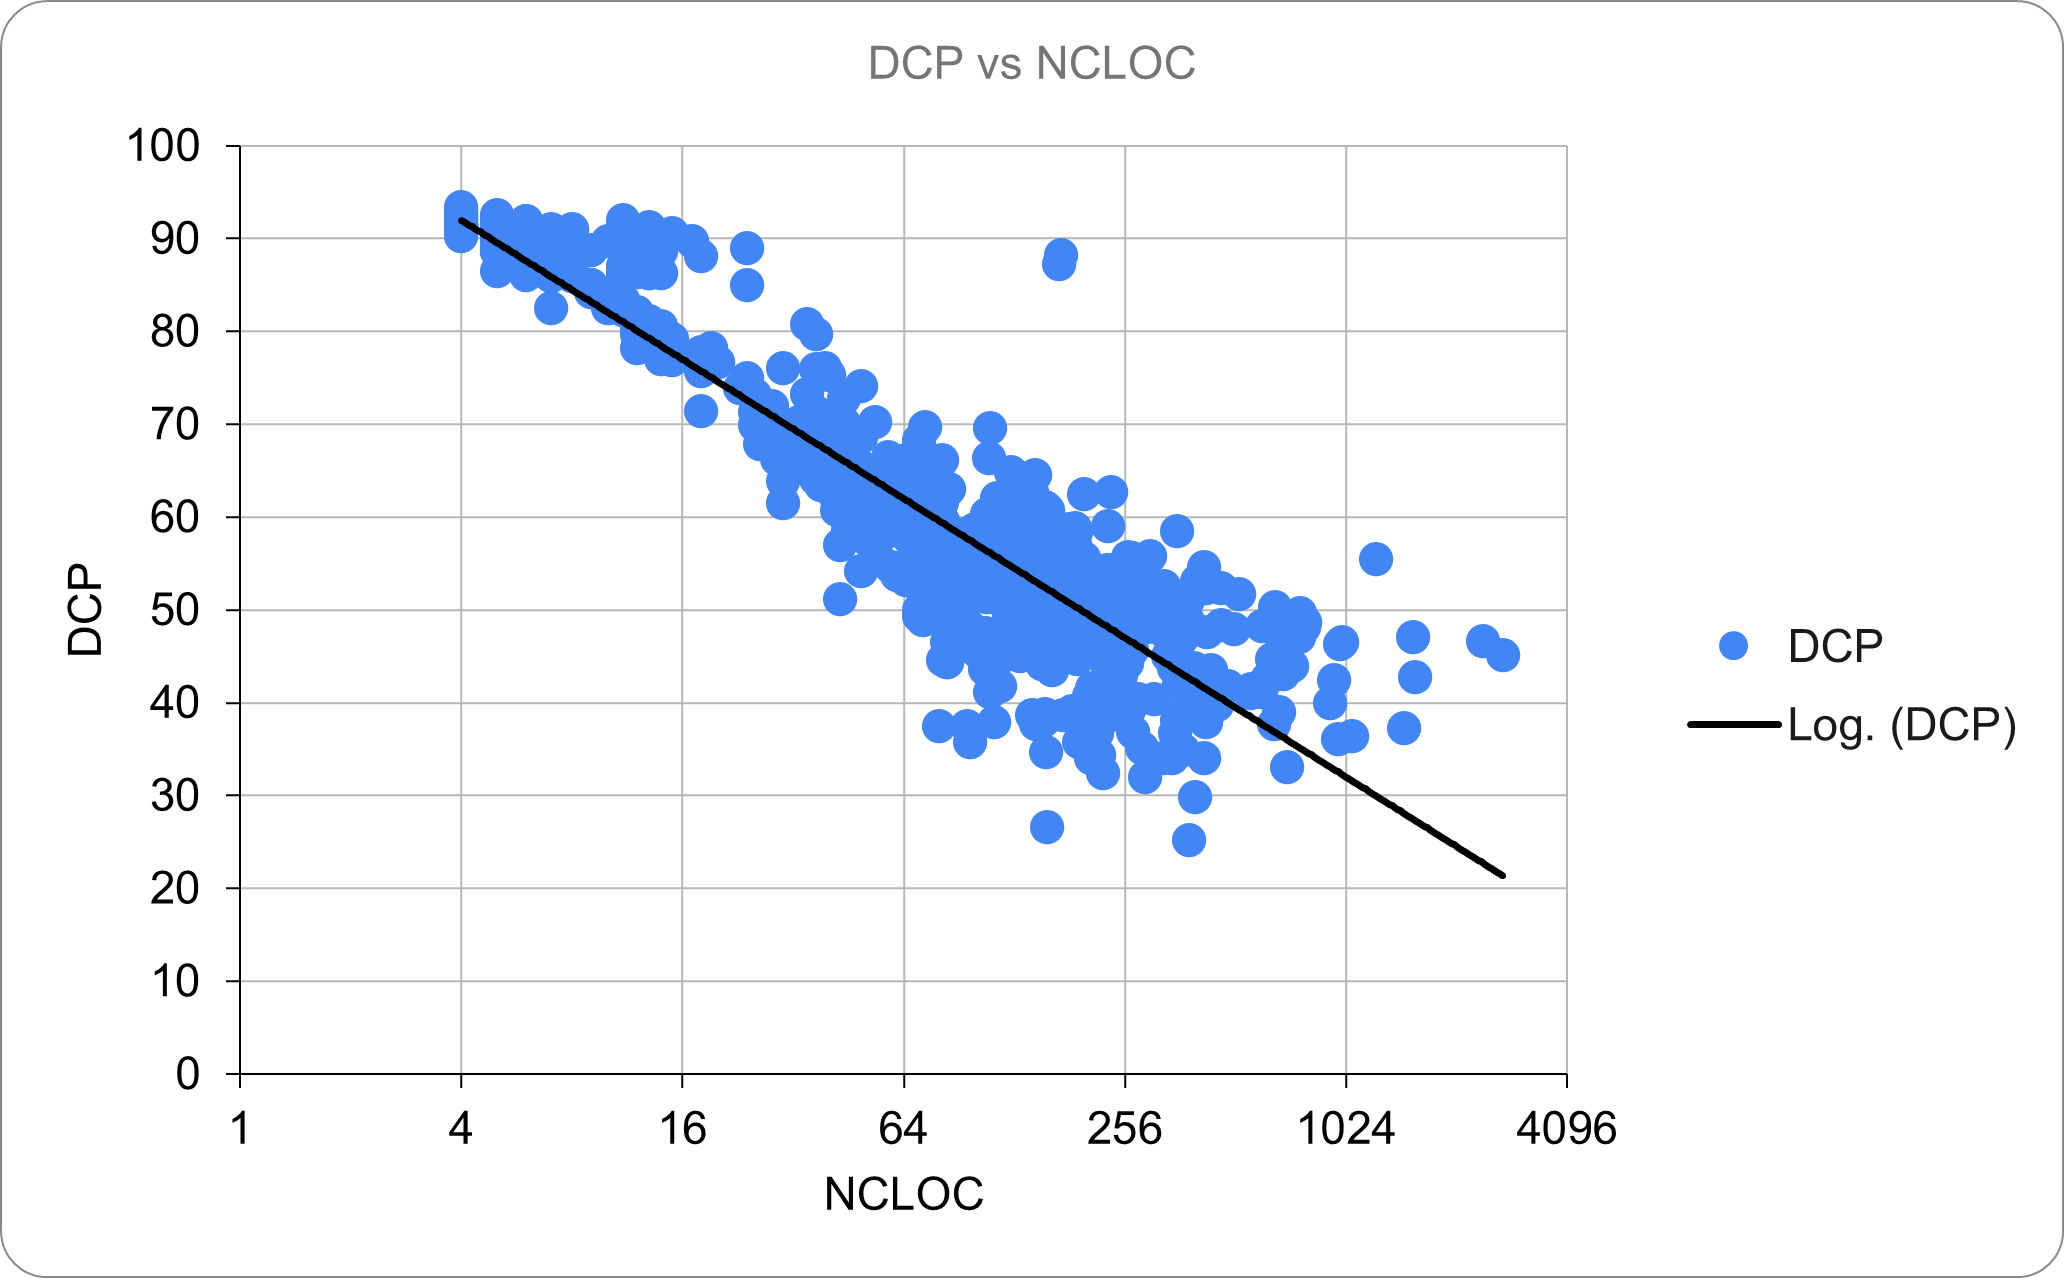
\includegraphics[width=0.33\linewidth, ]{figures/DCP vs NCLOC.png}
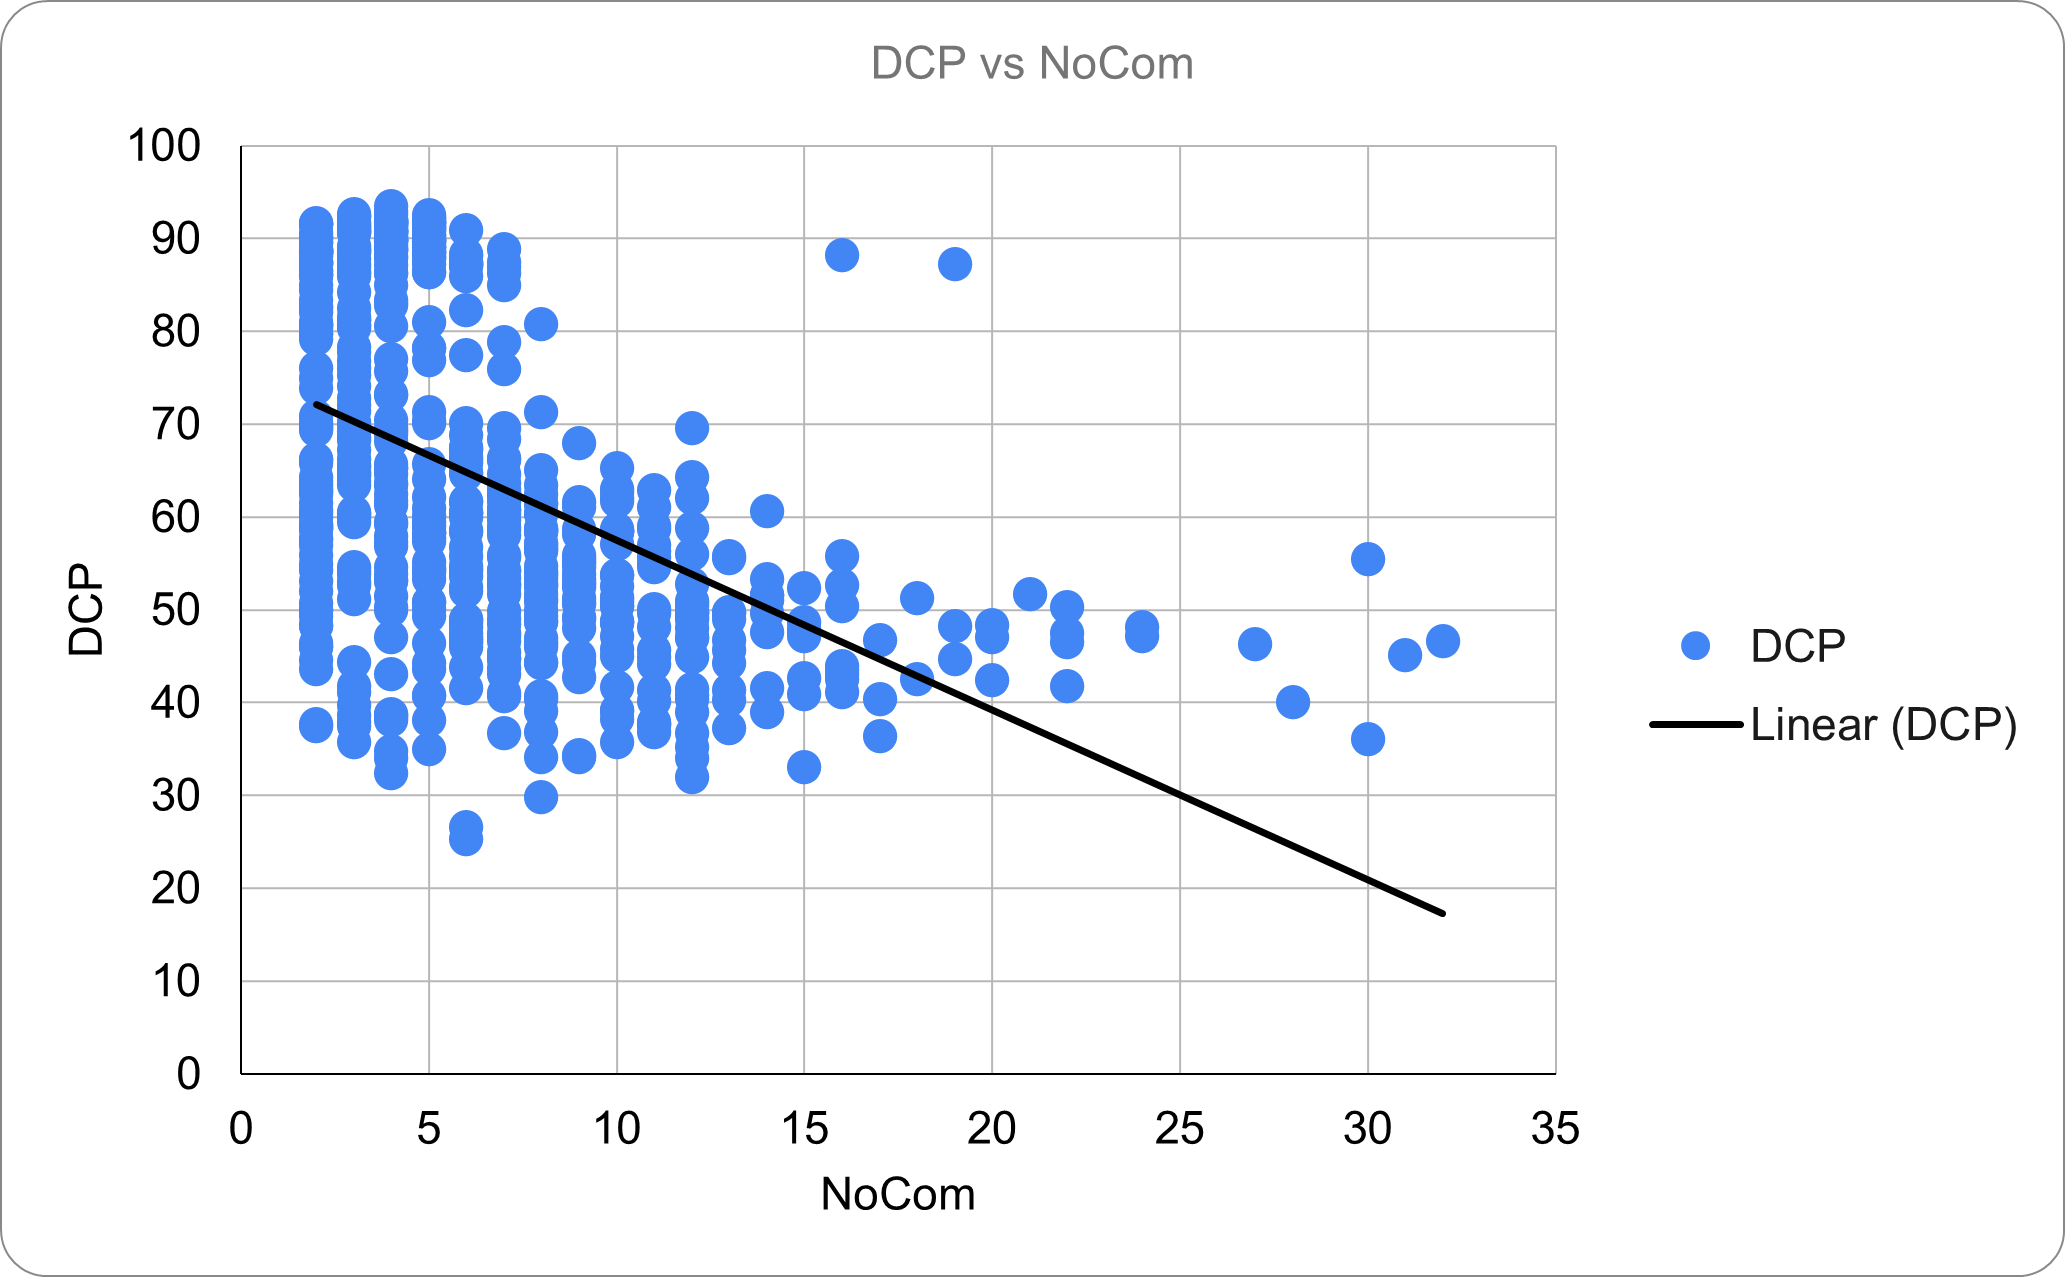
\includegraphics[width=0.33\linewidth]{figures/DCP vs NOCom.png}
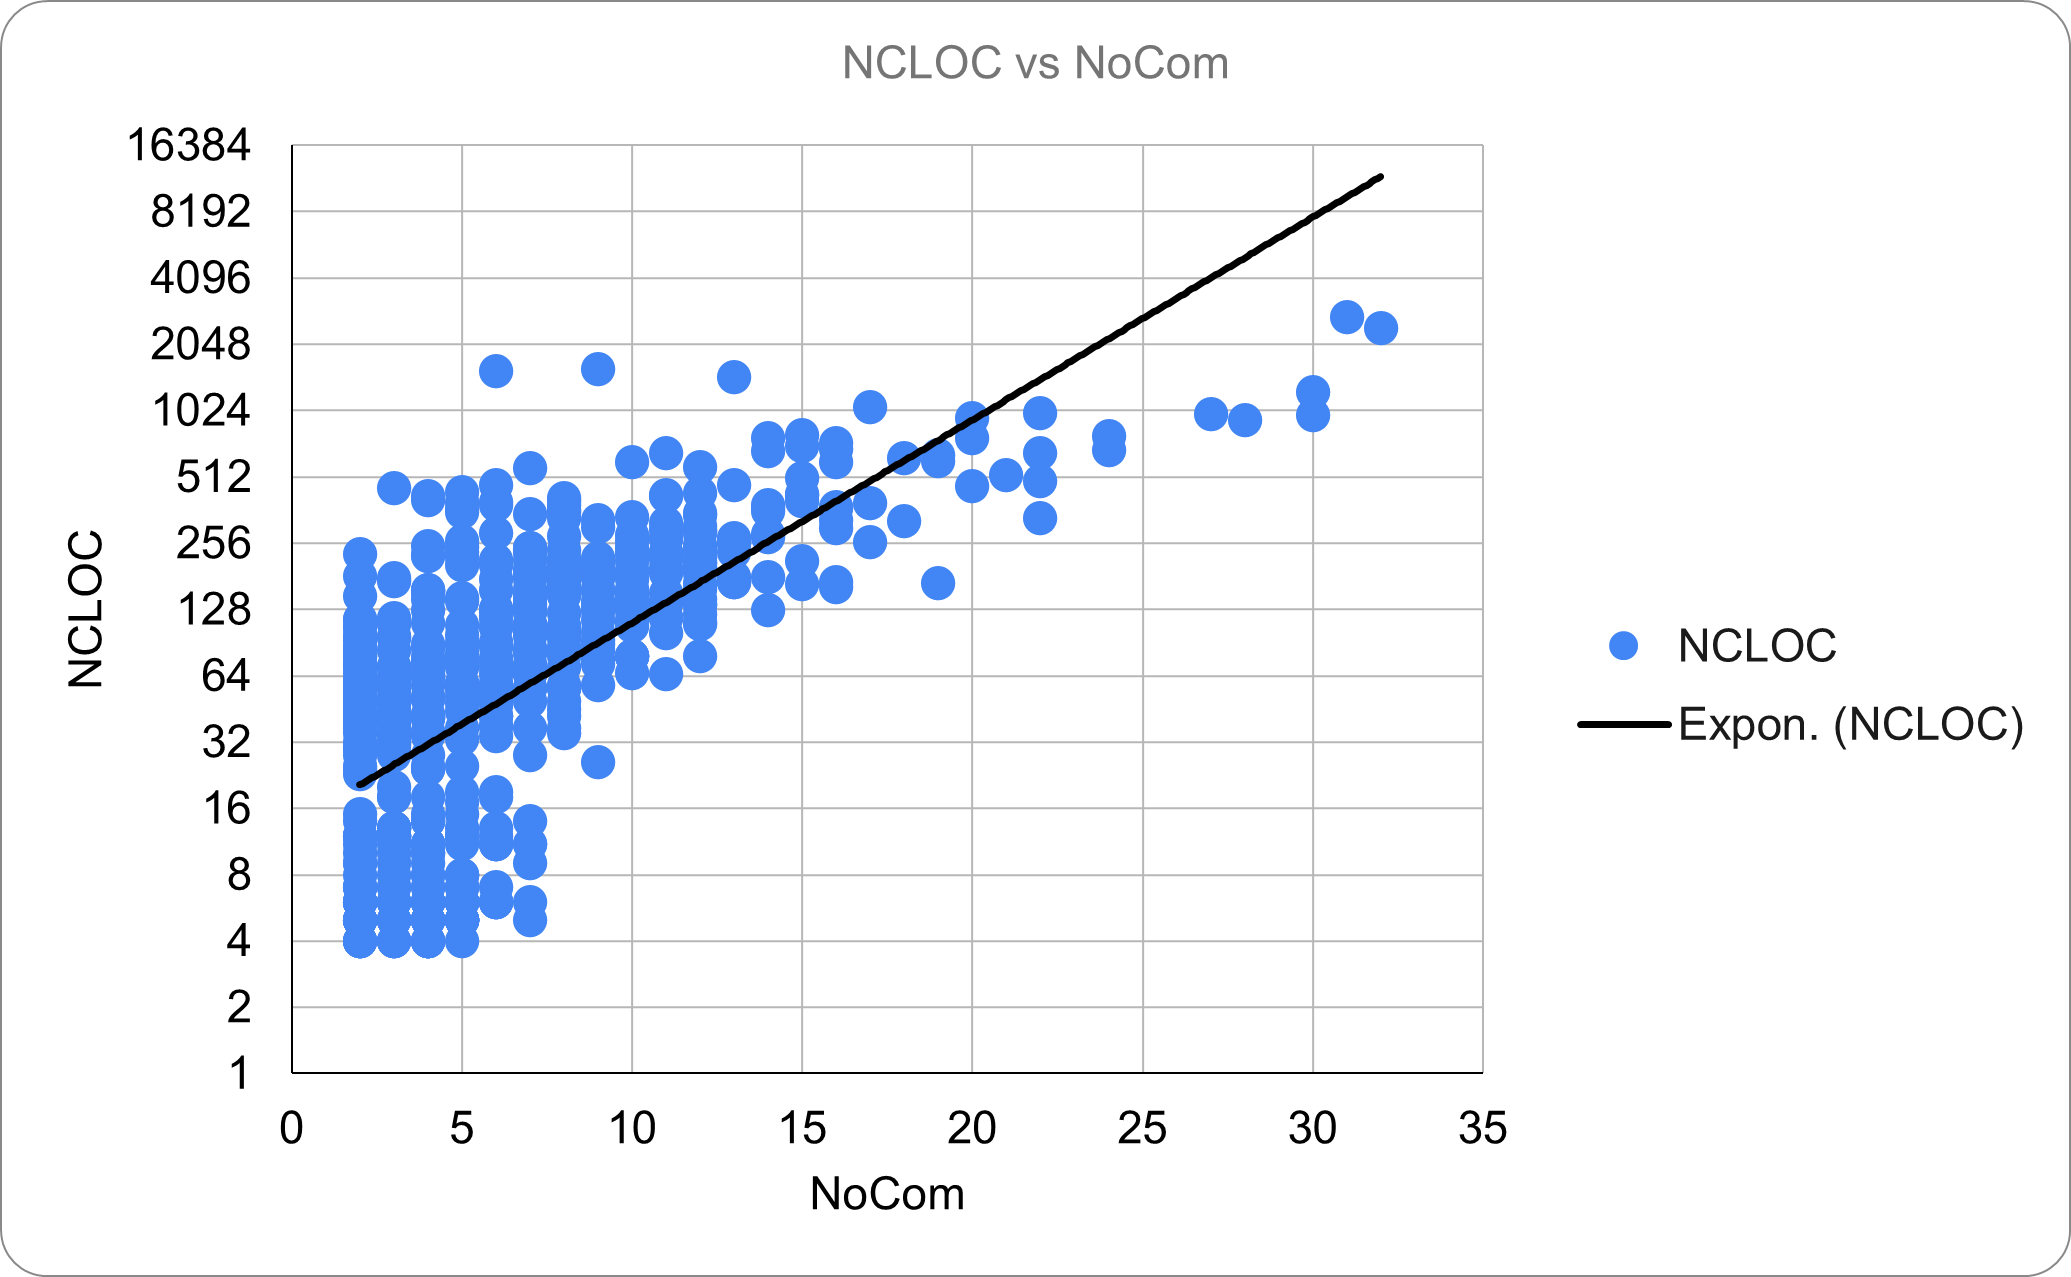
\includegraphics[width=0.33\linewidth]{figures/NCLOC vs NOCom.png}
\end{center}
Il nous faut maintenant déterminer si les variables sont normalement distribuées ou non.
À l'aide de graphiques composés avec Google Sheets, nous comparons la fréquence des données à leur courbe normale:\newline
\begin{center}
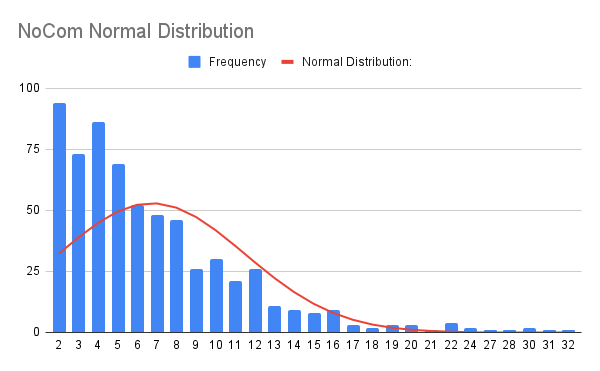
\includegraphics[width=0.33\linewidth]{figures/NoCom Normal Distribution.png}
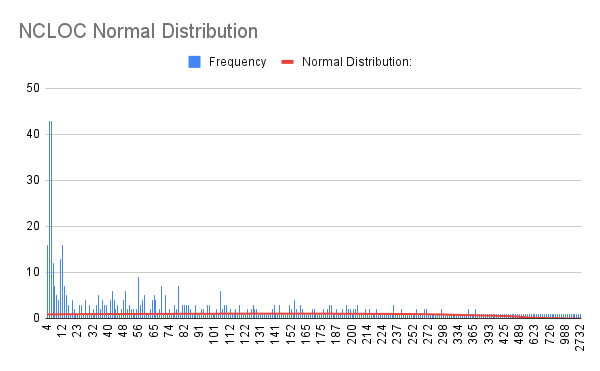
\includegraphics[width=0.33\linewidth]{figures/NCLOC Normal Distribution.png}
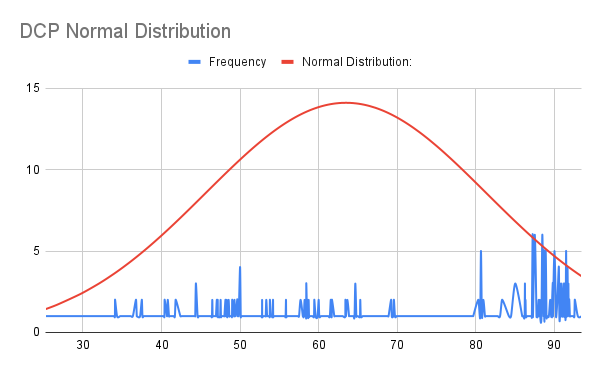
\includegraphics[width=0.33\linewidth]{figures/DCP Normal Distribution.png}
\end{center}
Il clair que ces variables ne sont fort probablement pas normalement distribuées.
Le coefficient de corrélation de Pearson (\emph{r}) ne peut être utilisé, car il exige une distribution normale.
Nous nous servirons donc du coefficient de corrélation de rang de Spearman ($\rho$), que nous calculons simplement en remplaçant nos valeurs par leur rang (RANK.AVG)
et en calculant ensuite \emph{r} sur ceux-ci en utilisant la fonction CORREL\footnote{https://support.google.com/docs/answer/3093990?hl=en}:
\begin{center}
NoCom vs NCLOC: $\rho$ = 0.69\hspace{1cm}
NoCom vs DCP: $\rho$ = -0.53\hspace{1cm}
NCLOC vs DCP: $\rho$ = -0.90
\end{center}
Nous voyons donc que NoCom et NCLOC ont une bonne corrélation positive, que NoCom et DCP ont une corrélation négative modérée
et que NCLOC et DCP ont une forte corrélation négative.

\vspace*{\fill}
\section{Partie 3 -- Hypothèse:}

Il nous faut finalement vérifier l'hypothèse suivante:
\begin{center}
    "\emph{Les classes qui ont été modifiées plus de 10 fois sont mieux commentées que celles qui ont été modifiées moins de 10 fois.}"
\end{center}

\subsection{Choix d'étude}
Nous voulons vérifier l'existence d'une relation hypothétique entre le NoCom d'une classe et son DCP.
Pour ce faire, nous allons mesurer le NoCom et DCP des classes d'une base de code non-triviale
et nous allons comparer le DCP des classes dont le NoCom > 10 à celui des classes dont le NoCom $\leq$ 10.
Le type d'étude que nous allons poursuivre est une quasi-expérience, puisqu'il est impossible de former un groupe de contrôle.

\subsection{Énoncé des hypothèses}
L’hypothèse que nous proposons est que dans une base de code, les classes dont le NoCom > 10 ont un DCP
moyen significativement supérieur à celui des classes dont le NoCom $\leq$ 10.

\subsection{Définition des variables}
Nous cherchons à mesurer l'effet du NoCom sur le DCP.
La variable indépendante est donc le NoCom des classes, et la variable dépendante est le DCP des classes.

\subsection{Expérience et résultats}
L'échantillon donné dans le fichier jfreechart-stats.csv contient déjà les valeurs de NoCom et DCP des classes d'une base de code de taille significative.
Nous nous en sommes déjà servi pour calculer la corrélation entre le NoCom et le DCP à la partie 2.
Nous effectuons des calculs supplémentaires dans Excel\footnotemark[1] afin de générer les boîtes à moustaches suivantes:\vspace{\baselineskip}

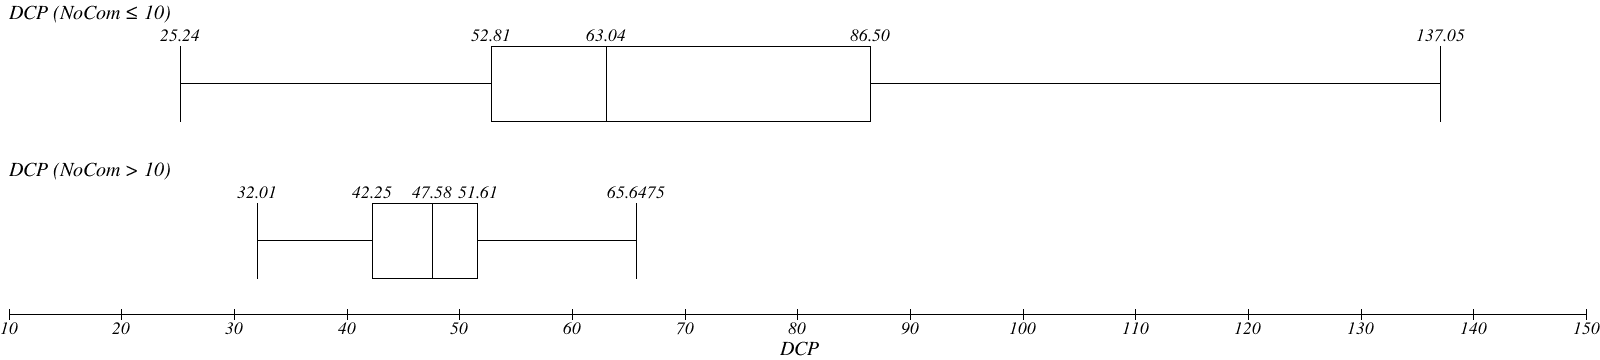
\includegraphics[width=\textwidth]{figures/t3nocom.png}\vspace{0.5em}

Celle du haut représente la distribution des valeurs de DCP des classes dont le NoCom est en-deçà de 10,
et celle du bas représente la distribution du DCP où le NoCom dépasse 10.

\subsection{Interprétation et généralisation des résultats}
Malgré la faiblesse de la corrélation entre le DCP et le NoCom, sa droite de régression ainsi que son coefficient de Spearman ($\rho$)
nous permet immédiatement de voir que le DCP tend plutôt vers le bas lorsque NoCom augmente, contrairement à l'hypothèse proposée.\vspace{0.5em}
\\
De plus, à part pour les 4 plus grande valeurs, la totalité des valeurs de DCP où NoCom > 10 se trouve en-deçà de la médiane de l'ensemble des valeurs de DCP où NoCom $\leq$ 10.
Ceci montre assez clairement que les classes qui ont été modifiées plus que 10 fois ne sont pas significativement mieux commentées
que les classes qui ont été modifiées moins que 10 fois. L'hypothèse ne peut donc être que fausse.\vspace{0.5em}
\\
À partir de la droite de régression, nous observons plutôt la tendance suivante: au fur et à mesure que NoCom augmente, DCP semble tendre vers 50\%.
En effet, alors que le DCP moyen des classes dont le NoCom $\leq$ 10 est de 66.6\%, celui des classes dont le NoCom > 10 est de 48.2\%.
Ceci peut s'expliquer par le fait que certains répositoires imposent ou encouragent un DCP minimum sur l'ensemble de leur code.
Si le DCP minimum de la base de code de JFreeChart est de 50\%, ceci expliquerait cette tendance.\vspace{0.5em}

\subsection{Discusssion des menaces à la validité}
Certains facteurs posent une menace à la validité de l’expérience.
Un tel facteur est que l’échantillon est sélectionné parmi une seule base de code écrit en un seul langage de programmation.
Ceci diminue considérablement la généralité des résultats, pour une multitude de raisons.\vspace{0.5em}
\\
Nous savons, par exemple, que les langages de haut niveau permettent au programmeur d'encoder plus instructions par ligne que les langages de bas niveau.
Alors, pour des fonctions équivalentes, un langage de bas niveau nécessite plus de lignes de code qu'un langage de haut niveau.
Ainsi, même si les lignes de commentaires reste le même, le DCP du langage de bas niveau sera plus bas que celui du langage de haut niveau.
Il est cependant clair que le code écrit dans le langage de haut niveau n'est tout de même pas mieux commenté que celui écrit dans un langage de bas niveau.

\end{document}